
Pour réaliser une étude sur différents isolants, une société réalise 3 maquettes de maison strictement identiques à l'exception près des isolants qui diffèrent dans chaque maquette. On place ensuite ces 3 maquettes dans une chambre froide réglée à 6 $^\circ$C. On réalise un relevé des températures ce qui permet de construire les 3 graphiques suivants: 

\begin{minipage}{0.48\linewidth}
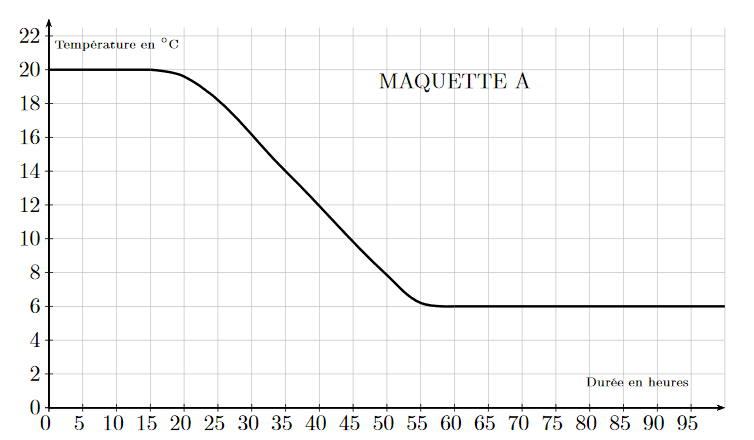
\includegraphics[scale=0.5]{NF-45-1.png} 
\end{minipage}
\hfill
\begin{minipage}{0.48\linewidth}
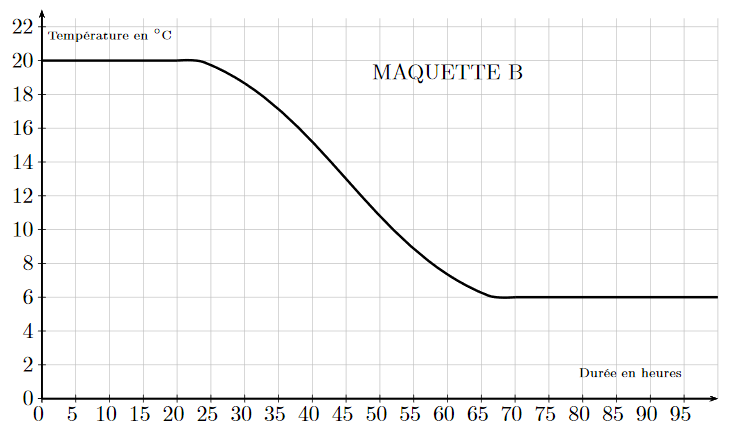
\includegraphics[scale=0.5]{NF-45-2.png} 
\end{minipage}

\begin{center}
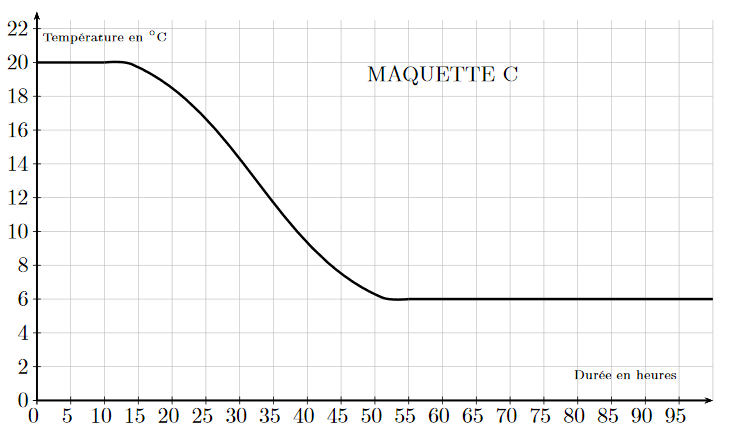
\includegraphics[scale=0.5]{NF-45-3.png} 
\end{center}

\medskip

\begin{enumerate}
\item  Quelle était la température des maquettes avant d'être mise dans la chambre froide? 

\item Cette expérience a-t-elle duré plus de 2 jours? Justifier votre réponse. 


\item Quelle est la maquette qui contient l'isolant le plus performant? Justifier votre réponse. 
\end{enumerate}
\medskip


\noindent \textbf{Partie 2 }: 

\noindent Pour respecter la norme RT2012 des maisons BBC (Bâtiments Basse Consommation), il faut que la résistance thermique des murs notée R soit supérieure ou égale à 4. Pour calculer cette résistance thermique, on utilise la relation: 

$$R=\dfrac{e}{c}$$ 

\noindent où $e$ désigne l'épaisseur de l'isolant en mètre et $c$ désigne le coefficient de conductivité thermique de l'isolant. Ce coefficient permet de connaître la performance de l'isolant. 

\begin{enumerate}
\item  Noa a choisi comme isolant la laine de verre dont le coefficient de conductivité thermique est: $c = 0,035$. Il souhaite mettre 15 cm de laine de verre sur ses murs. 

Sa maison respecte-t-elle la normé RT2012 des maisons BBC ? 

\item  Camille souhaite obtenir une résistance thermique de 5 ($R = 5$). Elle a choisi comme isolant du liège dont le coefficient de conductivité thermique est: $c = 0,04$. 

Quelle épaisseur d'isolant doit-elle mettre sur ses murs? 

\end{enumerate}